\documentclass[a4paper,12pt,oneside,headsepline]{scrreprt}
%\documentclass[a4paper,12pt,oneside,headsepline]{scrartcl}

\usepackage{ifxetex}
\ifxetex
	\usepackage{fontspec}
		\setmainfont{Gentium}
\fi

\usepackage{graphicx}
\usepackage{longtable}
\usepackage{tabularx}
\usepackage{setspace}
\usepackage{hyperref}
\usepackage{float}
\usepackage{flafter}
\usepackage{xcolor}
\usepackage{titlesec}
\usepackage{fancyhdr}

\pagestyle{fancy}


\hypersetup{%
    pdfborder = {0 0 0}
}

\addtokomafont{chapter}{\color[RGB]{83,88,85}}
\addtokomafont{section}{\color[RGB]{97,105,100}}

\KOMAoptions{parskip=half}
\KOMAoptions{DIV=12}

\onehalfspacing

\suppressfloats[t]
\suppressfloats[b]

%\clearscrheadfoot

%\ihead{Structured and Modular Design -> should be: current chapter}
%\ohead{Page \thepage\  of XXX}
\lhead{\nouppercase{\rightmark} (\nouppercase{\leftmark})}
\chead{}
\rhead{}

\renewcommand{\headrulewidth}{0.4pt}
\renewcommand{\footrulewidth}{0.4pt}

\renewcommand{\sectionmark}[1]{\markright{\MakeUppercase{#1}}{}}


\lfoot{Version 1.0}
\cfoot{\bfseries \thepage}
\rfoot{\today}

\fancypagestyle{plain}{%
\fancyhf{} % clear all header and footer fields
\fancyfoot[C]{\bfseries \thepage} % except the center
\fancyfoot[L]{Version 1.0}
\fancyfoot[R]{\today}
\fancyhead[LO,RE]{\slshape  \leftmark} %
\renewcommand{\headrulewidth}{0.4pt}
\renewcommand{\footrulewidth}{0.4pt}}

\subject{Software Engineering / Book Express}
\title{Structured and Modular Design}

\author{Christoph Wurm, Stefan Lenzen, Christian Hoff}
\date{\today}


\begin{document}
\pagenumbering{roman}
\maketitle
\newpage
\tableofcontents
\newpage
\listoftables
\newpage

\pagenumbering{arabic}
\setcounter{page}{4}

\section{Document history}
\begin{longtable}[c]{|p{0.20\textwidth}|p{0.22\textwidth}|p{0.35\textwidth}|p{0.1\textwidth}|}
\hline
Editor(s) & Date & Purpose of editing & Version\\
\hline
\hline
All & October, 16th 2009 & First draft & 0.1 \\
\hline
\caption{Document history}
\end{longtable}
\newpage
\section{Introduction}
The software architecture of a system is the set of structures needed to reason about the system, which comprise software elements, relations among them, and properties of both\footnote{\href{en.wikipedia.org/wiki/Software_architecture}{en.wikipedia.org/wiki/Software\_architecture}}.

All these elements shall be described in the following chapters. The method of \emph{Structured and Modular Design} will be used to describe the architecture of the program core. The operating system environment, including interfaces to existing software, will also be discussed.

The design specification is threefold: In the beginning, a high-level overview over the application design is provided and interfaces to existing programs are described.

Secondly, we will elaborate on the defined function modules. We will conclude with a description of the data modules. Thereby a \emph{Data Dictionary} will be used to outline the format of all stored application data.
\newpage
\section{Architectural overview}
As defined in the Software Requirement Specification by Team 2, a web interface will be provided for the customers of BookExpress. This includes both publishers and book stores. Publishers can use this interface to maintain a list of available book titles. For bookstores, the web interfaces provides a convenient way to order books and track the status of pending deliveries.

The web interface will be programmed using \emph{Java Enterprise Edition 6}.

A desktop application will be used by the employees of BookExpress. Compared to the web interface, it provides advanced functionality including the following:
\begin{itemize}
\item View the status of all pending orders
\item Starting the book delivery process
\item View business report and statistics
\end{itemize}

In addition a mobile client application is provided, which is going to be used by the employees working in the warehouse department. This system aims to support the employees during stock-keeping. It will pop up a notification whenever a book has been ordered. The application then shows the location of the ordered book in the warehouse such that the staff can easily find the ordered book. The software application will then ensure that one parcel is created for each bookstore, which contains the ordered books and an invoice.

\section{Interfaces to existing software}
The BookExpress software depends on other software products for some auxiliary functionality. The interfaces to these programs will be described in this chapter.
\subsection{DB2 database interface}
Certain data of the BookExpress software including customer and order information has to be stored in a persistent way. For this purpose, an existing database software will be used.

\emph{DB2} is a relational database software solution by IBM. We have chosen DB2 mainly because it focuses on business customers with high demands concerning performance, availability and support. It is also a mature programm which runs on many different platforms including(but not limited to) Linux, z/OS and Windows.

\emph{Java DataBase Connectivity(JDBC)} is a java binding which provides access to a wide range of relational databases including DB2. JDBC will serve as the binding between the BookExpress software and the database. Being a part of the Java framework, it also runs on every platform that is supported by Java.

\emph{Hibernate} is an object-relation model which maps entities in database tables to their corresponding Java classes. We will use Hibernate to make the database entities accessible in an object-oriented manner.
\subsection{TomTom navigation interface}
Usually a truck will deliver parcels to many bookstores, which makes a fast and efficient calculation of the delivery route necessary. For this reason, BookExpres relies on \emph{TomTom Navigator 7}, which will the route calculation and serve as a navigation system.

TomTom provides an \emph{Application Programming Interface(API)} which makes the functions of TomTom accessible to other programs. BookExpress will use this API in order to calculate the fastest route to the bookstores. As soon as a truck becomes available, the API enables the route to be trasnferred to this specific truck automatically.
\section{Design overview}
\begin{figure}[H]
\centering
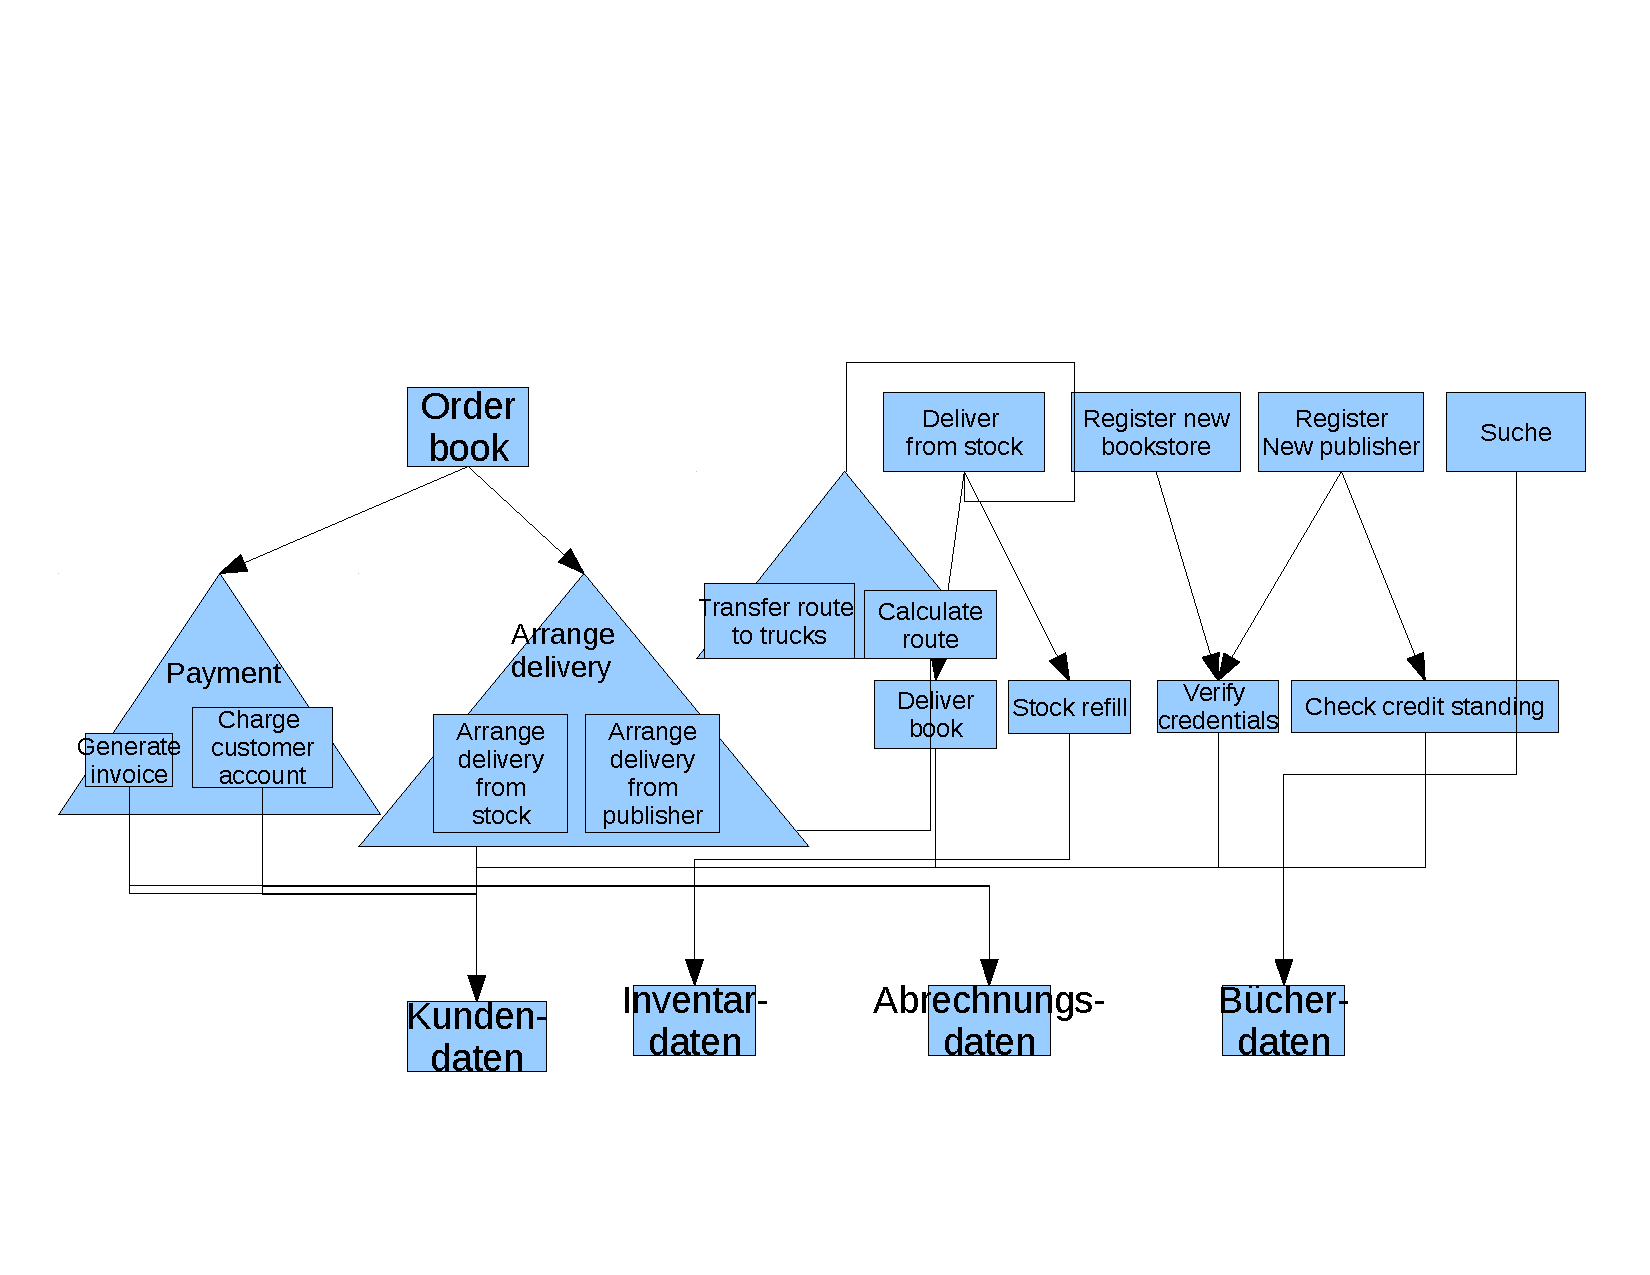
\includegraphics[scale=0.5]{design.pdf}
\caption{Modular design overview}
\end{figure}

\begin{longtable}[l]{|p{0.1\textwidth}|p{0.61\textwidth}|p{0.2\textwidth}|}
\hline
Number & Description & Reference to SRS  \\
\hline
\hline

DT0 & Ordering & \\
\hline
DT0.1 & Confirm order & \\
\hline
DT1 & Customer log-in & \\
\hline
DT2 & Select items & \\
\hline
DT3 & Check availability & \\
\hline

\caption{Decision Tables}
\end{longtable}
\end{document}
